\documentclass[12pt,a4paper]{article}
% Fix for fancyhdr headheight error
\setlength{\headheight}{14.5pt}
% --- PACKAGES ---
% --- ENCODING & FONTS ---
\usepackage[utf8]{inputenc}
\usepackage[T1]{fontenc}
\usepackage{lmodern}          % Modern font (alternative to Times)
% \usepackage{times}          % OPTIONAL: Classic serif font (comment if using lmodern)

\usepackage{pgf-pie}
\usepackage{pgfplots}
\usepackage{subcaption}
\usepackage{xcolor}
\usepackage{colortbl}
\usepackage{multirow}
\usepackage{booktabs}
\usepackage{siunitx}
\usepackage{float}

% --- PAGE LAYOUT ---
\usepackage[a4paper, left=0.75in, right=0.75in, top=1in, bottom=1in]{geometry}
\usepackage{parskip}          % Paragraphs with spacing instead of indentation
\usepackage{setspace}         % For line spacing

% --- MATHEMATICS ---
\usepackage{amsmath, amsfonts, amssymb}

% --- GRAPHICS & FIGURES ---
\usepackage{graphicx}
\usepackage{caption}
\usepackage{float}
\usepackage{array, longtable, colortbl}
\usepackage{tabularx}

% --- COLORS ---
\usepackage[table]{xcolor}
\usepackage{xcolor}           % General color usage

% --- TIKZ & DIAGRAMS ---
\usepackage{tikz}
\usetikzlibrary{
  shapes.geometric,
  arrows.meta,
  positioning,
  fit,
  backgrounds,
  shapes.multipart
}

% --- PLOTS & CHARTS ---
\usepackage{pgf-pie}          % Pie charts
\usepackage{pgfplots}         % Graphs and plots
% Set pgfplots compatibility for modern features
\pgfplotsset{compat=1.18}

% --- DOCUMENT STRUCTURE ---
\usepackage{titlesec}         % Custom section titles
\usepackage{tocloft}          % Table of contents formatting
\usepackage{enumitem}         % Better lists

% --- HEADER, FOOTER & LINKS ---
\usepackage{fancyhdr}         % Custom headers/footers

% --- BIBLIOGRAPHY ---
\usepackage[numbers,sort&compress]{natbib}  % For references with numerical citations
\bibliographystyle{plainnat}  % Compatible style with natbib
\usepackage[many]{tcolorbox}
\tcbuselibrary{skins,breakable}

% --- Code listings for source code in Appendix ---
\usepackage{listings}
\lstset{
    language=Python,
    basicstyle=\ttfamily\small,
    breaklines=true,
    showstringspaces=false,
    numbers=left,
    numberstyle=\tiny\color{gray},
    frame=single,
    captionpos=b,
    keywordstyle=\color{blue},
    commentstyle=\color{green!60!black},
    stringstyle=\color{purple},
    rulecolor=\color{black!20},
    backgroundcolor=\color{black!5}
}

% --- Load hyperref last ---
\usepackage{hyperref}         % Clickable links


% --- COLORS ---
\definecolor{RoyalBlue}{RGB}{0, 70, 140}
\definecolor{RUETRed}{RGB}{179, 0, 0}
\definecolor{LightGray}{RGB}{248, 249, 250}
\definecolor{DarkGray}{RGB}{52, 58, 64}
\definecolor{AccentBlue}{RGB}{13, 110, 253}
\definecolor{ModernGray}{RGB}{108, 117, 125}
\definecolor{lightgreen}{RGB}{200, 255, 200}
\definecolor{lightred}{RGB}{255, 200, 200}

% Define modern color palette
\definecolor{primary}{RGB}{41, 128, 185}
\definecolor{secondary}{RGB}{52, 152, 219}
\definecolor{accent}{RGB}{231, 76, 60}
\definecolor{success}{RGB}{46, 204, 113}
\definecolor{warning}{RGB}{241, 196, 15}
\definecolor{darkgray}{RGB}{52, 73, 94}
\definecolor{lightgray}{RGB}{236, 240, 241}
\definecolor{purple}{RGB}{155, 89, 182}
\definecolor{orange}{RGB}{230, 126, 34}
\definecolor{teal}{RGB}{26, 188, 156}
\definecolor{OliveGreen}{RGB}{85, 107, 47}

\definecolor{outputbg}{RGB}{45, 45, 45} % Dark background for output

% --> ADDED for the blue info box
% --> Define colors for code boxes and result boxes
\definecolor{reportgreen}{RGB}{230, 245, 230}
\definecolor{reportdarkgreen}{RGB}{50, 120, 50}
\definecolor{outputbg}{RGB}{45, 45, 45} % Dark background for output
\definecolor{infoboxbg}{RGB}{235, 245, 255}
\definecolor{infoboxborder}{RGB}{70, 130, 180}
% --> ADDED: Define the blue info box style
\newtcolorbox{infobox}{
  colback=infoboxbg,
  colframe=infoboxborder,
  boxrule=0.5pt, % thin border for sides/bottom
  borderline north={1.5pt}{0pt}{infoboxborder}, % thicker top border
  arc=0mm,       % sharp corners
  left=5mm, % Add some padding
  top=3mm,
  bottom=3mm
}

% --> Define style for code listings (like Listing 2, 3 in friend's report)
\lstdefinestyle{code}{
    basicstyle=\ttfamily\small,
    numbers=left,
    numberstyle=\tiny\color{gray},
    numbersep=5pt,
    frame=none,
    breaklines=true,
    keywordstyle=\color{blue},
    commentstyle=\color{OliveGreen},
    stringstyle=\color{purple},
    showstringspaces=false
}
\lstset{style=code} % Set default listing style

% --> Define the green result box
\newtcolorbox{resultbox}[2][]{
    enhanced,
    attach boxed title to top center={yshift=-2mm},
    colback=reportgreen,
    colframe=reportdarkgreen,
    colbacktitle=reportgreen,
    coltitle=black,
    boxed title style={size=small,colframe=reportdarkgreen},
    title={#2},
    fonttitle=\bfseries
}

% --- FONT & STYLING ---
\renewcommand{\familydefault}{\sfdefault}  % Use sans-serif font
\titleformat{\section}{\fontsize{20}{24}\selectfont\bfseries\color{RoyalBlue}}{\thesection}{1em}{}
\titleformat{\subsection}{\fontsize{16}{20}\selectfont\bfseries\color{RoyalBlue}}{\thesubsection}{1em}{}
\titleformat{\subsubsection}{\fontsize{13}{16}\selectfont\bfseries\color{RoyalBlue}}{\thesubsubsection}{1em}{}

% TOC Styling
\renewcommand{\cfttoctitlefont}{\color{black}\Huge\bfseries}
\renewcommand{\cftsecfont}{\color{RoyalBlue}}
\renewcommand{\cftsecpagefont}{\color{RoyalBlue}}
\renewcommand{\cftsubsecfont}{\color{RoyalBlue}}
\renewcommand{\cftsubsecpagefont}{\color{RoyalBlue}}

% Header and Footer
\pagestyle{fancy}
\fancyhf{}
\fancyhead[C]{\textit{Compiler Design Sessional}}
\fancyfoot[C]{\thepage}
\renewcommand{\headrulewidth}{0.4pt}
\renewcommand{\footrulewidth}{0pt}

% Hyperlink Styling
\hypersetup{
    colorlinks=true,
    linkcolor=RoyalBlue,
    filecolor=magenta,
    urlcolor=cyan,
    pdftitle={Data Mining Report},
    pdfpagemode=FullScreen,
    pdfborder={0 0 0},
}

% --- Define a global style for all plots for consistency ---
\pgfplotsset{
    every axis/.append style={
        axis x line=bottom,
        axis y line=left,
        label style={font=\bfseries},
        title style={font=\large\bfseries, yshift=1em},
        tick label style={font=\small},
        legend style={font=\small, at={(0.5,-0.2)}, anchor=north, legend columns=-1},
    }
}

% Modern title page with geometric design
\newcommand{\maketitlepage}{
    \begin{titlepage}
        \begin{tikzpicture}[remember picture,overlay]
            \fill[RoyalBlue!10] (current page.north west) rectangle ([yshift=-2.2cm]current page.north east);
            \fill[AccentBlue!5] ([yshift=-14cm]current page.north west) rectangle ([yshift=-16.2cm]current page.north east);
            \fill[RoyalBlue!15] ([xshift=2cm,yshift=-2cm]current page.north west) circle (1.2cm);
            \fill[AccentBlue!15] ([xshift=-2cm,yshift=-15.2cm]current page.north east) circle (0.9cm);
        \end{tikzpicture}

        \centering
        \vspace*{0.6cm}

        % Logo (only include if file exists)
        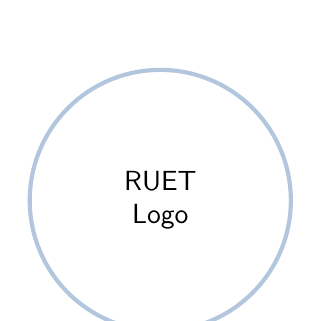
\begin{tikzpicture}
            \node[circle, draw=RoyalBlue!30, line width=1.5pt, inner sep=6pt] at (0,0) {
                 \IfFileExists{RUET_logo.png}{\includegraphics[width=2.7cm]{RUET_logo.png}}{\begin{minipage}{2.7cm}\centering RUET \\ Logo \end{minipage}}
            };
        \end{tikzpicture}

        \vspace{0.6cm}
        {\fontsize{15.5}{17}\selectfont\bfseries\textcolor{RUETRed}{RAJSHAHI UNIVERSITY OF ENGINEERING \& TECHNOLOGY}\par}
        \vspace{0.2cm}
        {\fontsize{13.5}{16}\selectfont\textcolor{DarkGray}{Department of Computer Science and Engineering}\par}

        \vspace{1.5cm}
        % Title Block
        
\begin{tikzpicture}
            \node[rectangle, fill=RoyalBlue!5, rounded corners=12pt, inner sep=12pt, text width=11.5cm, align=center] at (0,0) {
                {\fontsize{21}{24}\selectfont\bfseries\textcolor{RoyalBlue}{Lab Evaluation 1 Report}\par}
                \vspace{0.15cm}
                {\fontsize{16}{20}\selectfont\bfseries\textcolor{DarkGray}{-}\par}
                \vspace{0.15cm}
                {\fontsize{24}{28}\selectfont\bfseries\textcolor{AccentBlue}{"Compiler Design"}\par}
            };
        \end{tikzpicture}

        \vspace{1.8cm}
        % Submission info
        \begin{minipage}[t]{0.45\textwidth}
            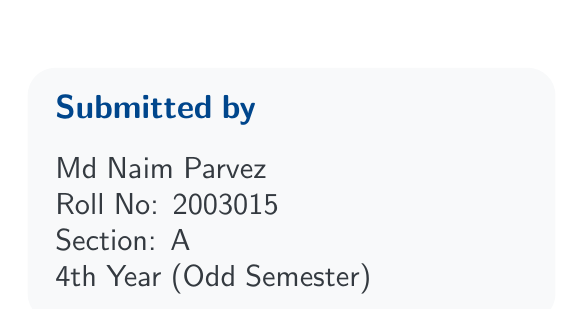
\begin{tikzpicture}
                \node[rectangle, fill=LightGray, rounded corners=10pt, inner sep=10pt, text width=6cm] at (0,0) {
                    {\fontsize{13}{15}\selectfont\bfseries\textcolor{RoyalBlue}{Submitted by}\par}
                    \vspace{0.3cm}
                    {\fontsize{11}{13}\selectfont\textcolor{DarkGray}{
                        Md Naim Parvez\\
                        Roll No: 2003015\\
                        Section: A\\
                        4th Year (Odd Semester)
                    }\par}
                };
            \end{tikzpicture}
        \end{minipage}
        \hfill
        \begin{minipage}[t]{0.50\textwidth}
            
\begin{tikzpicture}
                \node[rectangle, fill=AccentBlue!5, rounded corners=10pt, inner sep=10pt, text width=6cm] at (0,0) {
                    {\fontsize{13}{15}\selectfont\bfseries\textcolor{RoyalBlue}{Submitted to}\par}
                    \vspace{0.3cm}
                    {\fontsize{11}{13}\selectfont\textcolor{DarkGray}{
                        Farjana Parvin\\
                        Assistant Professor\\
                        Department of CSE\\
                        Rajshahi University of Engineering \& Technology\\
                        \vspace{0.3cm}
                    }\par}
                };
            \end{tikzpicture}
        \end{minipage}

        \vspace{1.2cm}
        % Course Info
        
\begin{tikzpicture}
            \node[rectangle, fill=RoyalBlue!10, rounded corners=10pt, inner sep=12pt, align=center, text width=13cm] at (0,0) {
                {\fontsize{13}{16}\selectfont\bfseries\textcolor{RoyalBlue}{Course Code: } \textcolor{DarkGray}{4102}}\\[0.2cm]
                {\fontsize{13}{16}\selectfont\bfseries\textcolor{RoyalBlue}{Course Title: } \textcolor{DarkGray}{Compiler Design Sessional}}
            };
        \end{tikzpicture}

        \vspace{0.8cm}
    \end{titlepage}
}


\begin{document}

% --- TITLE PAGE ---
\maketitlepage
\thispagestyle{empty} % No header/footer on the title page

\newpage
% --- TABLE OF CONTENTS ---
\pagenumbering{roman} % Roman numerals for ToC, Abstract etc.
\phantomsection % Helps hyperref create proper links
\tableofcontents

% --- LIST OF FIGURES ---
\newpage
\phantomsection % Helps hyperref create proper links
\pagenumbering{arabic} % Arabic numerals for main content
\setcounter{page}{1} % Start main content page numbering from 1
% ============= CHAPTER 1: INTRODUCTION =============
\section{Introduction}

\section{Objective}
The objective of this laboratory exercise is to understand the compilation process in C programming, specifically focusing on generating object files using the GNU Compiler Collection (GCC). This experiment demonstrates the use of Makefiles for automated compilation and the generation of object files with the extension \texttt{.o}.

\section{Theory}

\subsection{Compilation Process}
The C compilation process consists of four main stages:
\begin{enumerate}
    \item \textbf{Preprocessing:} Handles directives like \texttt{\#include} and \texttt{\#define}
    \item \textbf{Compilation:} Converts preprocessed code to assembly language
    \item \textbf{Assembly:} Converts assembly code to machine code (object file)
    \item \textbf{Linking:} Links object files with libraries to create executable
\end{enumerate}

\subsection{Object Files}
An object file (\texttt{.o} extension) contains machine code but is not yet executable. It requires linking with system libraries and other object files to create a final executable program. The \texttt{-c} flag in GCC instructs the compiler to stop after the assembly stage and produce an object file.

\subsection{Makefile}
A Makefile is a build automation tool that contains rules for compiling and linking programs. It helps manage dependencies and automates the build process, making it easier to compile complex projects with multiple source files.

\section{Problem Statement}
Given a simple C program that calculates the sum of two integers, generate an object file named \texttt{question1.objectfile.o} using a Makefile. The Makefile should contain only the necessary commands for compilation without any extra or redundant commands.

\section{Source Code}

\subsection{C Source File (question1.c)}
\begin{lstlisting}[language=C, caption={question1.c - Simple Addition Program}]
#include <stdio.h>  
int main() { 
    int num1 = 5; 
    int num2 = 10; 
    int sum = num1 + num2; 
    printf("The sum is: %d\n", sum);  
    return 0; 
}
\end{lstlisting}

\subsection{Makefile}
\begin{lstlisting}[language=make, caption={Makefile for Object File Generation}]
all:
	gcc -c question1.c -o question1.objectfile.o
\end{lstlisting}

\section{Methodology}

\subsection{Steps Performed}
\begin{enumerate}
    \item Created the source file \texttt{question1.c} with the given C program
    \item Created a \texttt{Makefile} with a single compilation rule
    \item Executed the command \texttt{make} or \texttt{make all} in the terminal
    \item Verified the generation of \texttt{question1.objectfile.o}
    \item Examined the object file properties and contents
\end{enumerate}

\subsection{Compilation Command Explanation}
The GCC command used in the Makefile:
\begin{verbatim}
gcc -c question1.c -o question1.objectfile.o
\end{verbatim}

\textbf{Command breakdown:}
\begin{itemize}
    \item \texttt{gcc}: The GNU C Compiler
    \item \texttt{-c}: Compile and assemble, but do not link (generates object file)
    \item \texttt{question1.c}: Input source file
    \item \texttt{-o}: Specify output file name
    \item \texttt{question1.objectfile.o}: Output object file name
\end{itemize}

\section{Execution and Results}

\subsection{Compilation Output}
When executing \texttt{make} command in the terminal:
\begin{verbatim}
$ make
gcc -c question1.c -o question1.objectfile.o
$
\end{verbatim}

The compilation completed successfully without any errors or warnings.

\subsection{Generated Object File}
After successful compilation, the following file was generated:
\begin{itemize}
    \item \textbf{Filename:} question1.objectfile.o
    \item \textbf{File Type:} ELF 64-bit relocatable object file (on Linux systems)
    \item \textbf{File Size:} Approximately 1.5-2 KB (varies by system)
\end{itemize}

\subsection{Verification Commands}
To verify the object file generation and examine its properties:

\begin{lstlisting}[language=bash, caption={Verification Commands}]
# List the generated object file
$ ls -lh question1.objectfile.o
-rw-r--r-- 1 user user 1.6K Dec 12 12:00 question1.objectfile.o

# Check file type
$ file question1.objectfile.o
question1.objectfile.o: ELF 64-bit LSB relocatable, x86-64

# Display object file symbols
$ nm question1.objectfile.o
0000000000000000 T main
                 U printf
\end{lstlisting}

\subsection{Program Execution}
To create an executable from the object file and run the program:
\begin{verbatim}
$ gcc question1.objectfile.o -o program
$ ./program
The sum is: 15
\end{verbatim}

The program successfully calculated the sum of 5 and 10, displaying the output: \texttt{The sum is: 15}

\section{Analysis and Discussion}

\subsection{Makefile Analysis}
The provided Makefile is minimal and contains only the necessary command to generate the object file. It follows the requirement of having no extra or redundant commands:

\begin{itemize}
    \item Single target: \texttt{all}
    \item Single compilation command using GCC
    \item Uses the \texttt{-c} flag to generate object file only
    \item Specifies custom output filename with \texttt{.objectfile.o} extension
\end{itemize}

\subsection{Object File Contents}
The generated object file contains:
\begin{itemize}
    \item Machine code for the \texttt{main()} function
    \item Symbol table with defined and undefined symbols
    \item Relocation information for the \texttt{printf()} function
    \item Section headers for code, data, and debugging information
\end{itemize}

\subsection{Key Observations}
\begin{enumerate}
    \item The object file is \textbf{not executable} on its own
    \item It contains unresolved references (like \texttt{printf}) that need linking
    \item The file is platform-specific (architecture and OS dependent)
    \item The \texttt{-c} flag prevents automatic linking, creating only the object file
\end{enumerate}

\section{Advantages of Using Makefiles}
\begin{itemize}
    \item \textbf{Automation:} Simplifies the build process with a single command
    \item \textbf{Consistency:} Ensures the same compilation flags are used every time
    \item \textbf{Efficiency:} In larger projects, Make only recompiles changed files
    \item \textbf{Maintainability:} Centralized build configuration
    \item \textbf{Portability:} Same Makefile can work across different systems
\end{itemize}

\section{Possible Errors and Troubleshooting}
\begin{itemize}
    \item \textbf{Syntax Errors:} Missing semicolons or braces in C code
    \item \textbf{Makefile Tab Issues:} Makefiles require actual tab characters, not spaces
    \item \textbf{File Not Found:} Ensure question1.c exists in the same directory
    \item \textbf{Permission Issues:} May need write permissions in the directory
    \item \textbf{Compiler Not Found:} GCC must be installed on the system
\end{itemize}

\section{Conclusion}
This laboratory exercise successfully demonstrated the generation of object files using the GCC compiler and Makefiles. The experiment covered:

\begin{itemize}
    \item Understanding the compilation process and the role of object files
    \item Creating a minimal Makefile for automated compilation
    \item Using the \texttt{-c} flag to generate object files without linking
    \item Verifying the generated object file and understanding its properties
    \item Recognizing that object files are intermediate files in the compilation process
\end{itemize}

The Makefile contained only the necessary command to compile the source file into an object file, adhering to the requirement of avoiding extra or redundant commands. The generated \texttt{question1.objectfile.o} file was successfully created and later linked to produce a working executable that correctly calculated and displayed the sum of two integers.

\section{Learning Outcomes}
\begin{enumerate}
    \item Understood the distinction between compilation and linking stages
    \item Learned to use GCC flags effectively, particularly the \texttt{-c} flag
    \item Gained practical experience with Makefile creation and usage
    \item Understood the structure and purpose of object files
    \item Recognized the importance of build automation in software development
\end{enumerate}

\end{document}